\documentclass[11pt,a4paper,titlepage]{scrartcl}

\usepackage{harvard}
%notwendiges Package f\"ur Journal of Finance Bibliostyle
%\usepackage{babelbib}
\usepackage{graphicx}
\usepackage{setspace}
\usepackage[english]{babel}
\usepackage{amsmath}
%\usepackage{times}
\usepackage{booktabs}
\usepackage[utf8]{inputenc}

\usepackage{geometry}
\geometry{a4paper, top=30mm, left=30mm, right=30mm, bottom=30mm}




%kann angeschaltet werden, falls Times Schrift erw\"unscht
\usepackage{array}
\usepackage{tabularx}
\usepackage{dcolumn}
\usepackage{longtable}
\usepackage{colortbl}
\usepackage{rotating}
\usepackage{multirow}
\usepackage{scrlayer-scrpage}
\usepackage{nameref}
\usepackage{amsfonts}


\usepackage{txfonts} %Schriftart Times New Roman
\usepackage{ulem} %added by me
\usepackage{caption}  % added by me for text in table
\usepackage{placeins} %added by me Include this for \FloatBarrier
\usepackage{float} % Added by me to 'fix' tables



\pagestyle{scrheadings} 
\clearpairofpagestyles
\rohead{\headmark}                                   

 

\linespread{1.5}
%Stellt Zeilenabstand ein
\setlength{\footheight}{20.40001pt} 
\setlength{\headheight}{20.40001pt}

%BEGIN DOCUMENT%%%%%%%%%%%%%%%%%%%%%%%%%%%%%%%%%%%%%%%%%%%%%%%%%%

\begin{document} 


\newpage

\thispagestyle{plain}
\begin{titlepage}

\begin{center}

\huge{\textbf{Flash loans in ethereum using Aave}}\\[1.5ex]
\LARGE{Different use cases with specific analysis of applications}\\[6ex]
\Large{Advanced Studies in Finance / Sustainable Finance Master Thesis 
Finance Executive Education  \\
Finance Weiterbildung}\\[1.5ex]
\Large{Dr. Benjamin Wildiing}\\
\Large{Manuel Keller}\\[12	ex]


\end{center}


\normalsize
\begin{flushleft}
Written by:\\[3ex]
Andrea Merli\\[1ex]
Plattenstrasse 14\\[1ex]
8302 Zürich\\[3ex]

Filling date: XX.Januar.20YY\\[10ex]
\end{flushleft}

\begin {figure}[h]
\begin {center}

\includegraphics [width=4.5cm] {uzh_logo_d_pos.eps}
\end {center}
\end {figure}


\end{titlepage}


%Der folgende Abschnitt erm\"oglicht das einf\"ugen von der eingescannten Aufgabenstellung (hier drei Seiten) Scale und Ordnerangabe (Zusatz/AuftragX) muss an die jeweiligen Bed\"urfnisse angepasst werden.
%\markboth{}{Aufgabenstellung}
%\cfoot{}
%\begin{center}
%\includegraphics[scale=0.73]{Zusatz/Auftrag1}

%\includegraphics[scale=0.73]{Zusatz/Auftrag2}

%\includegraphics[scale=0.73]{Zusatz/Auftrag3}

%\end{center}
\pagenumbering{Roman}
\cfoot{\pagemark}
\newpage
%\pagenumbering{Roman}
\section*{Abstract}
\normalsize
abstract abstract abstract abstract abstract abstract abstract abstract abstract abstract abstract abstract abstract abstract abstract abstract abstract abstract abstract abstract abstract abstract abstract abstract abstract abstract abstract abstract abstract abstract abstract abstract abstract abstract abstract abstract. abstract abstract abstract abstract abstract abstract abstract abstract abstract abstract abstract abstract abstract abstract abstract abstract abstract abstract abstract abstract abstract abstract abstract abstract abstract abstract abstract abstract abstract abstract abstract abstract abstract abstract abstract abstract abstract abstract abstract abstract abstract abstract abstract abstract abstract abstract abstract abstract abstract abstract abstract abstract abstract abstract abstract abstract abstract abstract abstract abstract abstract abstract abstract abstract abstract abstract abstract abstract abstract .

\newpage





\tableofcontents

\newpage

\listoffigures

\newpage

\listoftables

\newpage
\section*{Abbreviations}

\newpage

\pagenumbering{arabic}

%%%%%%%%%%%%%%%%%%%%%%%%%%% EINLEITUNG
\section{Einleitung \label{sect:Introduction}}
\subsection{Ausgangslage und Problemstellung}
\subsection{Ziel der Arbeit}
\subsection{Aufbau und Vorgehen}
\subsection{Abgrenzungen}

\section{Aave protocol}
\subsection{Aave lending protocol basics}
Aave is one of the most used and battle tested lending protocols in DeFi. Before Aave version 1 (V1) there were other solutions for decentralised lending strategy, among them, ethlend which has been founded by the same team and it is the natural Aave precursor; ethlend was  peer to peer (P2P), resulting in a direct lender - borrower matching handled by a smart contract. A traditional finance instrument to represent this is an OTC contract, represented in figure \ref{fig:peer_lending} to which the decentralized finance (DEFI) community added, at first, a layer for decentralisation and peers matching. The P2P approach enables  the credit process in a decentralised environment but is not flexible and is illiquid cause the charged rate and lended amount in a potential loan must be published waiting for an interested counterpart. 
\begin{figure}[ht]
    \centering
    \begin{minipage}[t]{0.45\textwidth} % Adjust width as needed
        \centering
        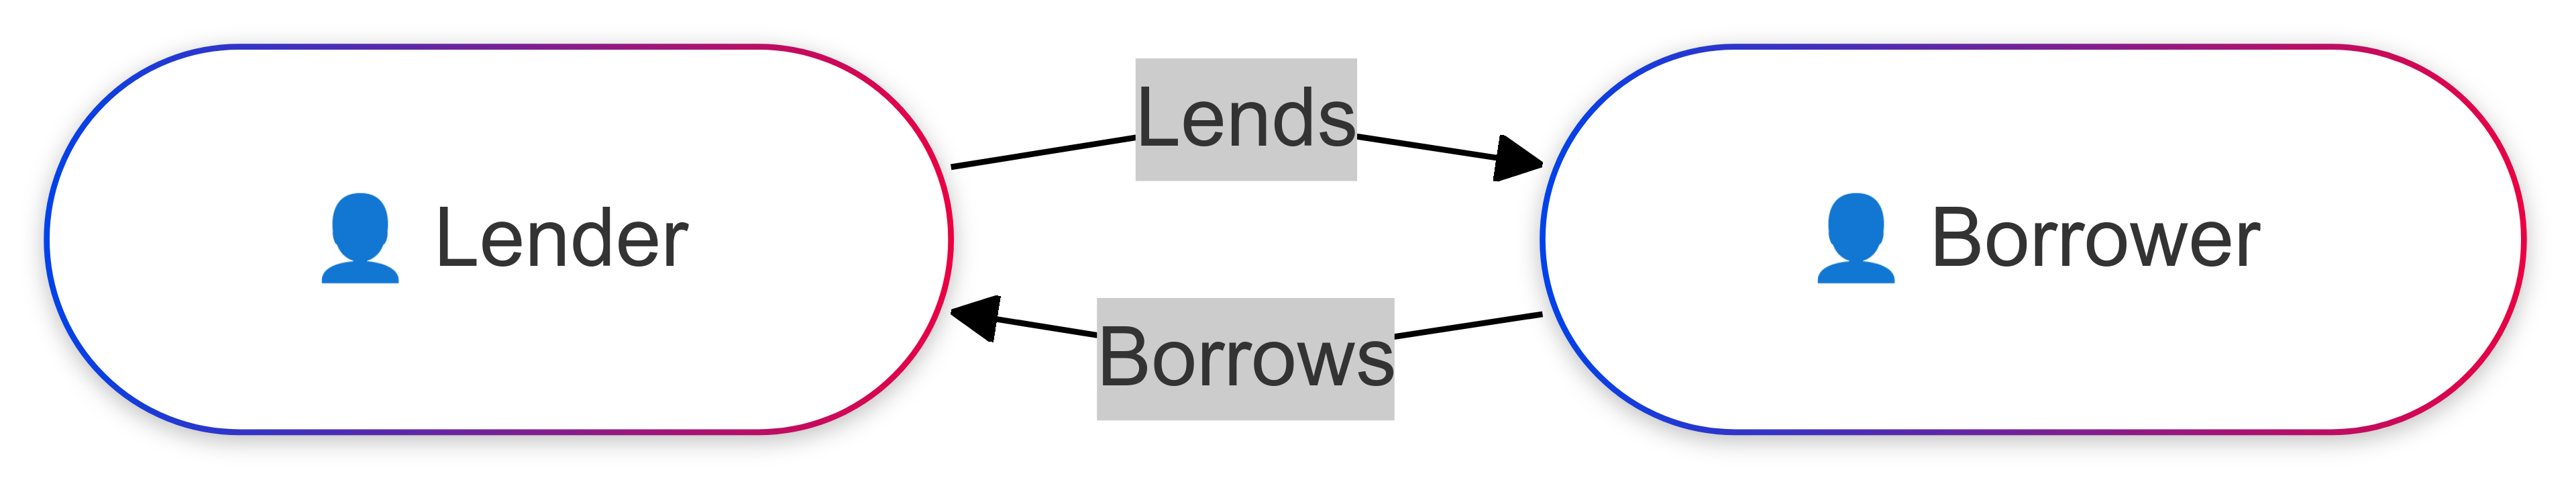
\includegraphics[width=\textwidth]{image/otclendborrow.png}
        \caption{P2P lending borrowing (OTC)}
        \label{fig:peer_lending}
    \end{minipage}
    \hfill % Horizontal space between the figures
    \begin{minipage}[t]{0.45\textwidth} % Adjust width as needed
        \centering
        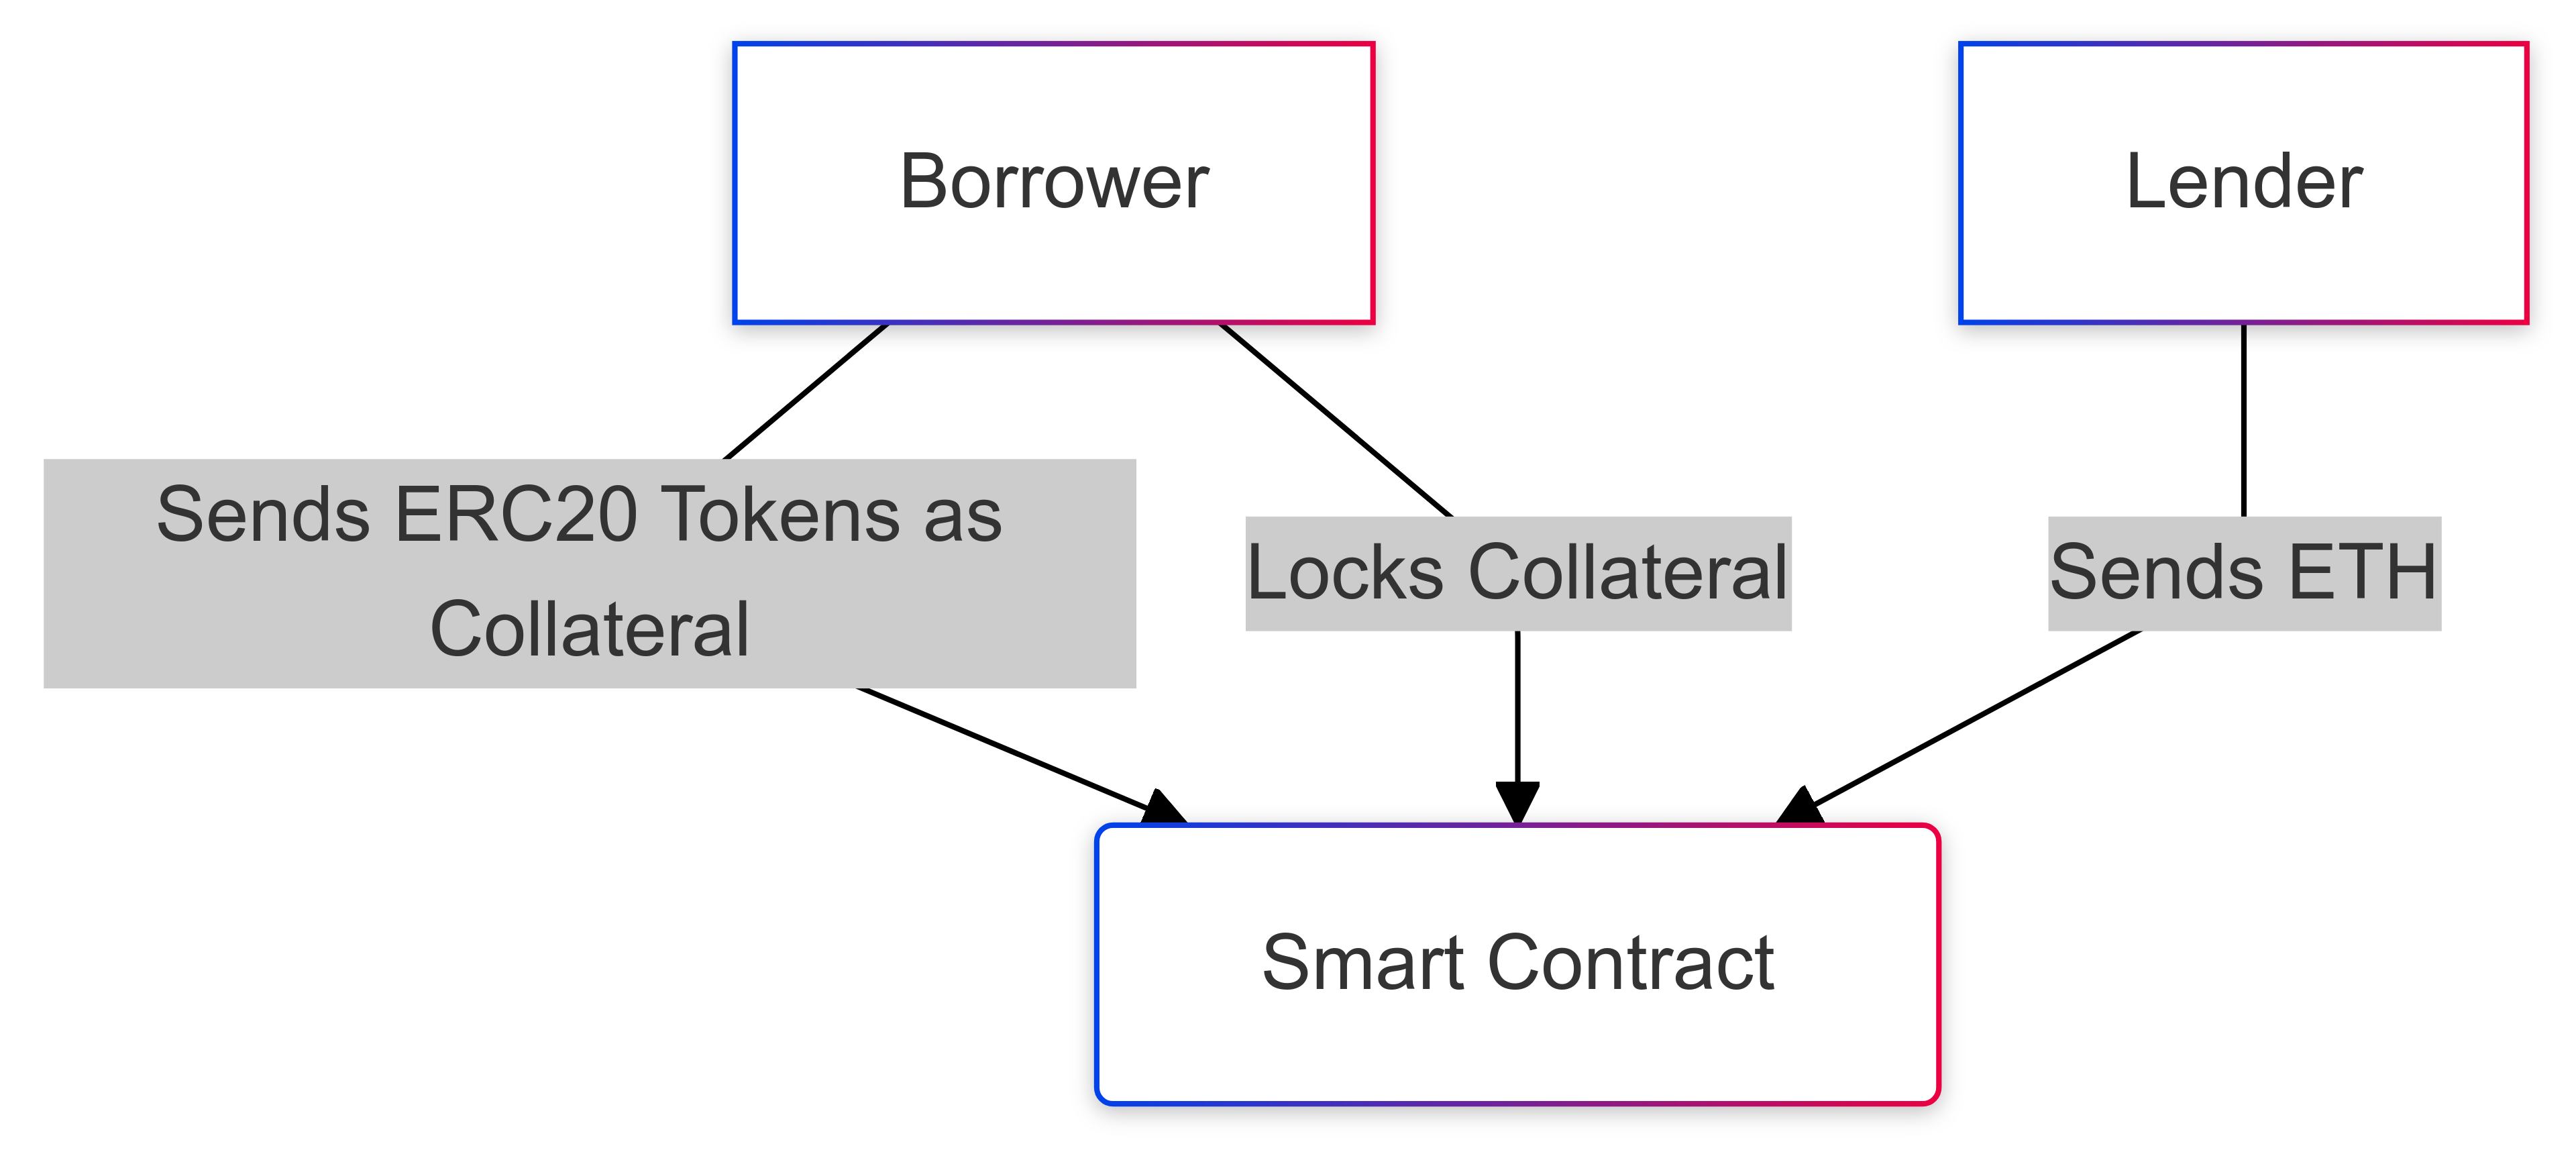
\includegraphics[width=\textwidth]{image/lenderborrowerOTC}
        \caption{smart contract handling lender borrowed P2P interaction}
        \label{fig:lending_contract}
    \end{minipage}
    \FloatBarrier
\end{figure}

In detail the OTC solution  provided by ethLend, represented in figure \ref{fig:lending_contract}, consists in a lender borrower smart contract interaction where  borrowers create a loan request  posting  ERC-20 compatible tokens  as collateral and setting  the loan’s length, interest premium and the amount of tokens needed for collateral. If a lender agrees to these terms, a loan agreement will be created.
There are only two possible outcomes: if the borrower repays the loan, the lender then receives his or her original principal plus interest and the borrower takes back the collateral which is unlocked from the smart contract whereas if the borrower fails to repay his or her loan, the lender will receive the borrower’s posted collateral. 

\begin{figure}[ht]
    \centering
    \begin{minipage}[t]{0.53\textwidth} % Adjust width as needed
        \centering
        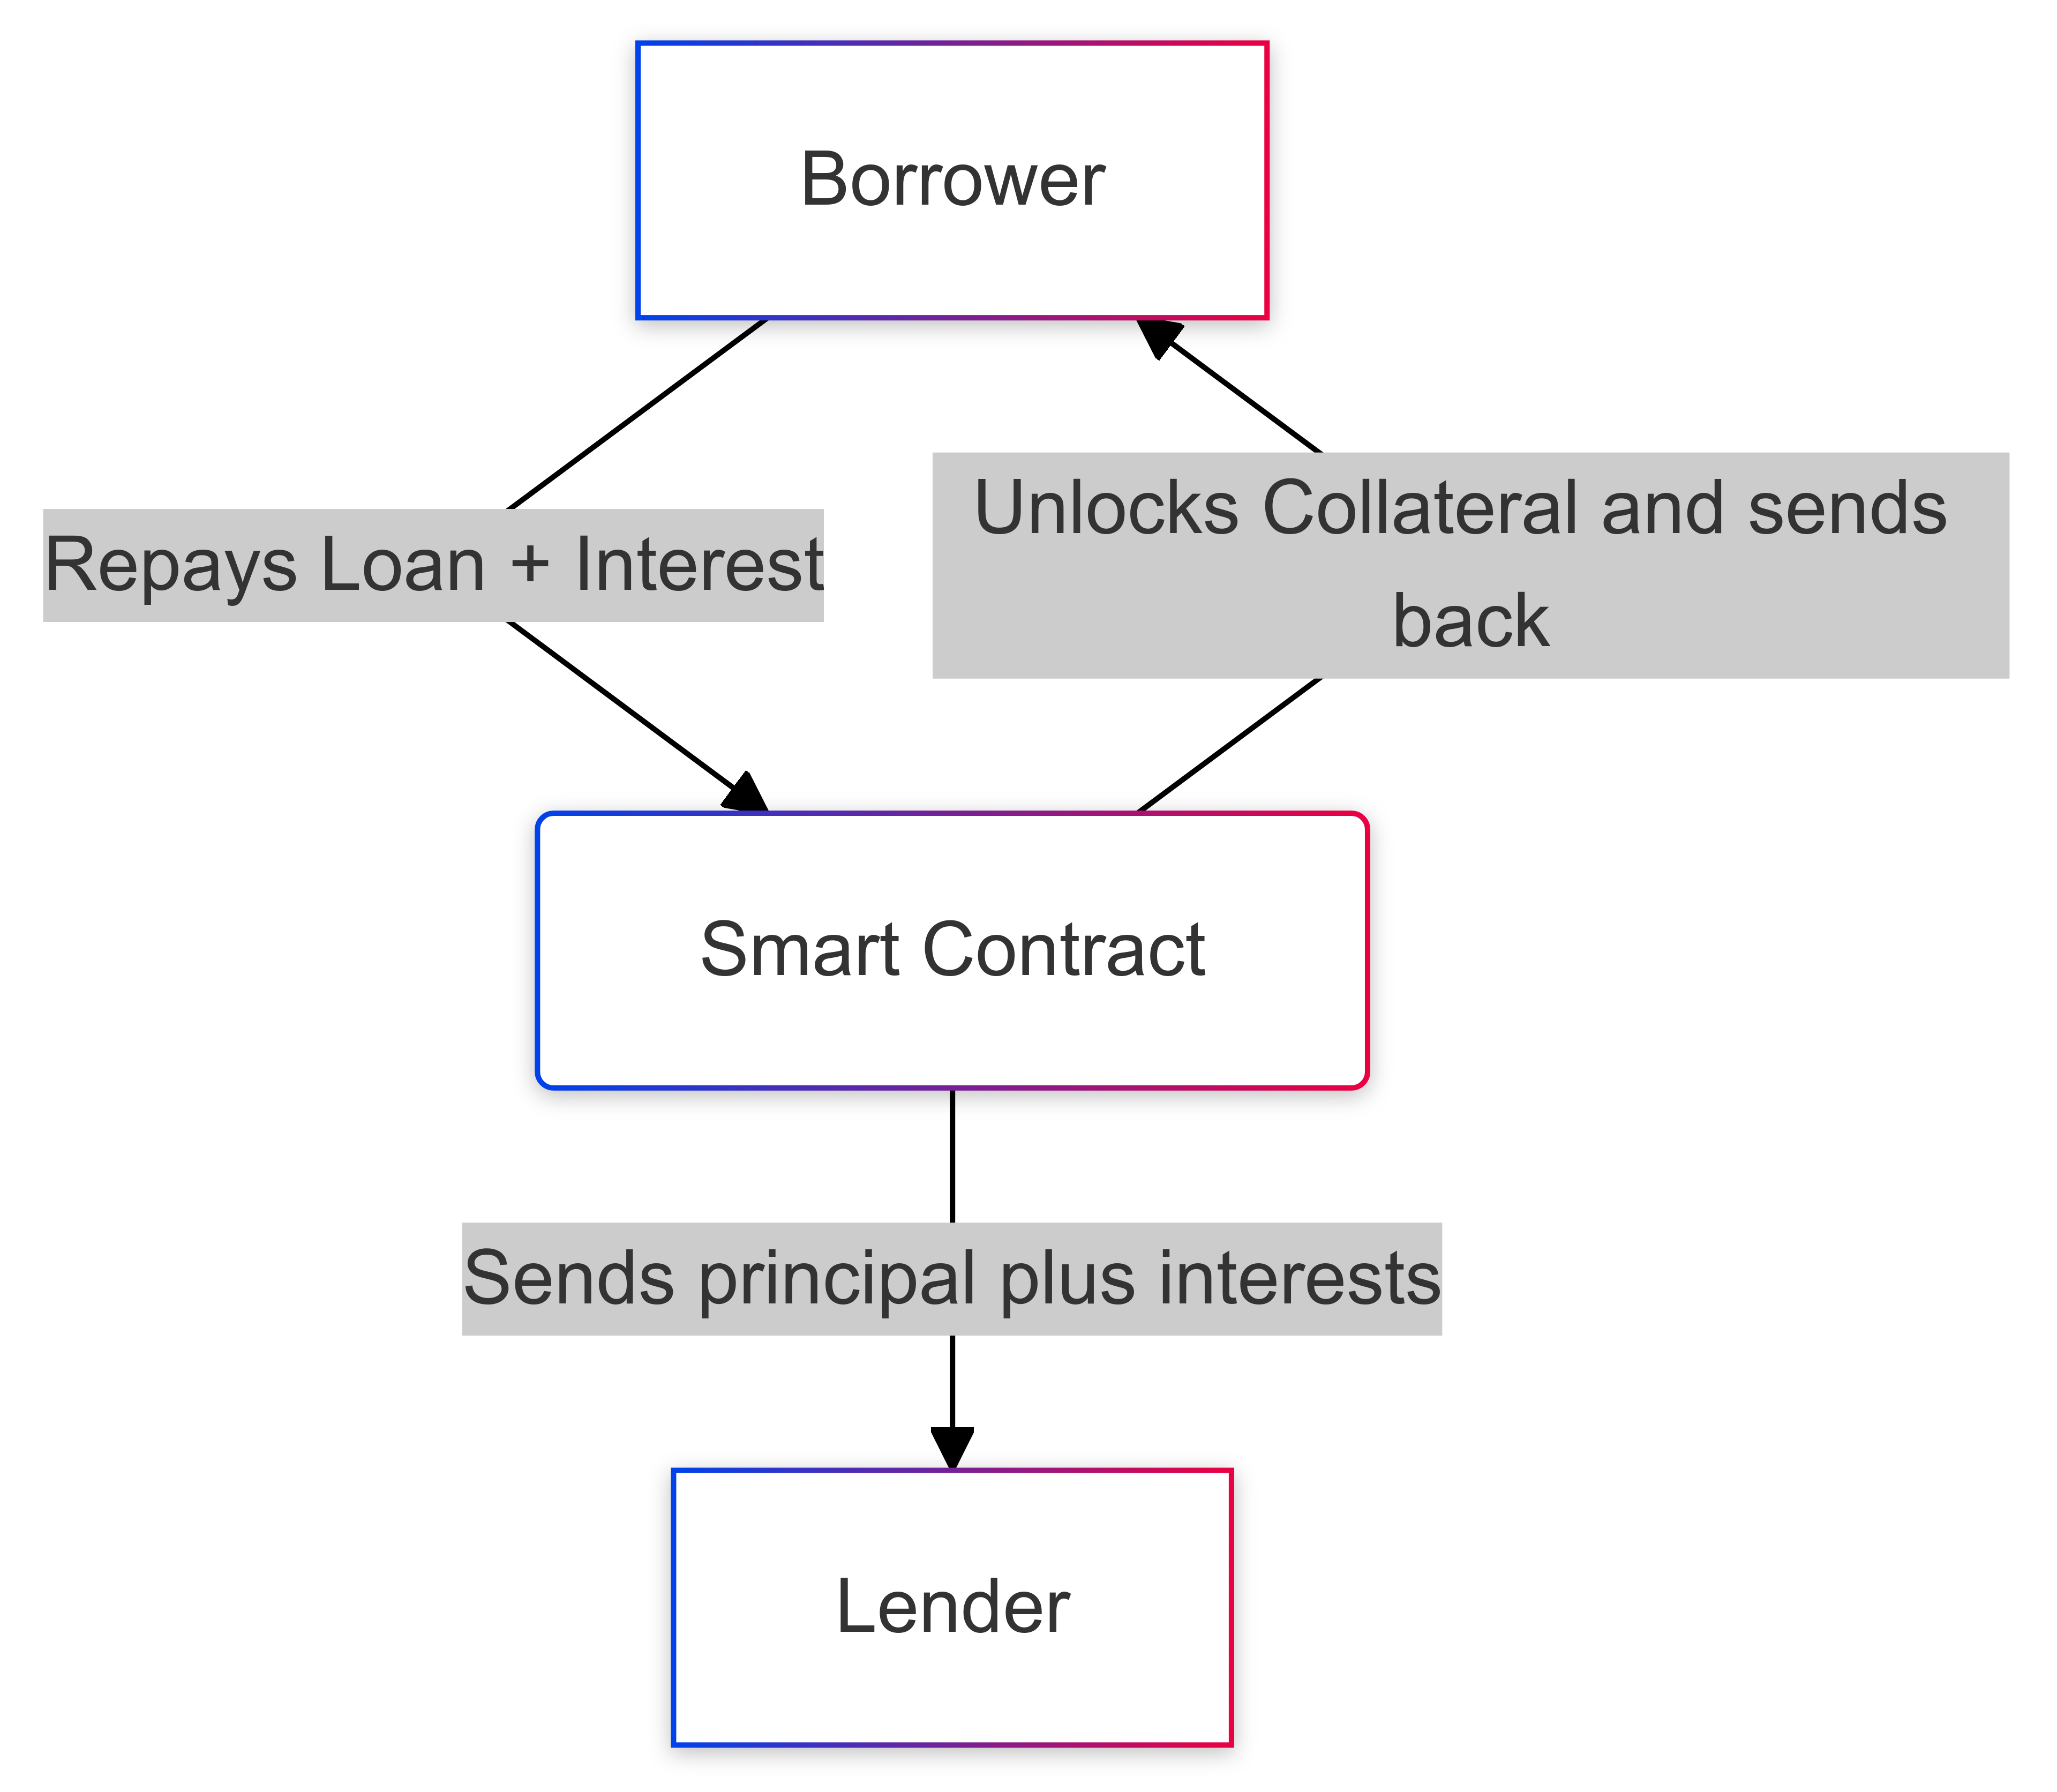
\includegraphics[width=\textwidth]{image/otcrepayment}
        \caption{Borrower repays the loan}
        \label{fig:repays}
    \end{minipage}
    \hfill % Horizontal space between the figures
    \begin{minipage}[t]{0.3\textwidth} % Adjust width as needed
        \centering
        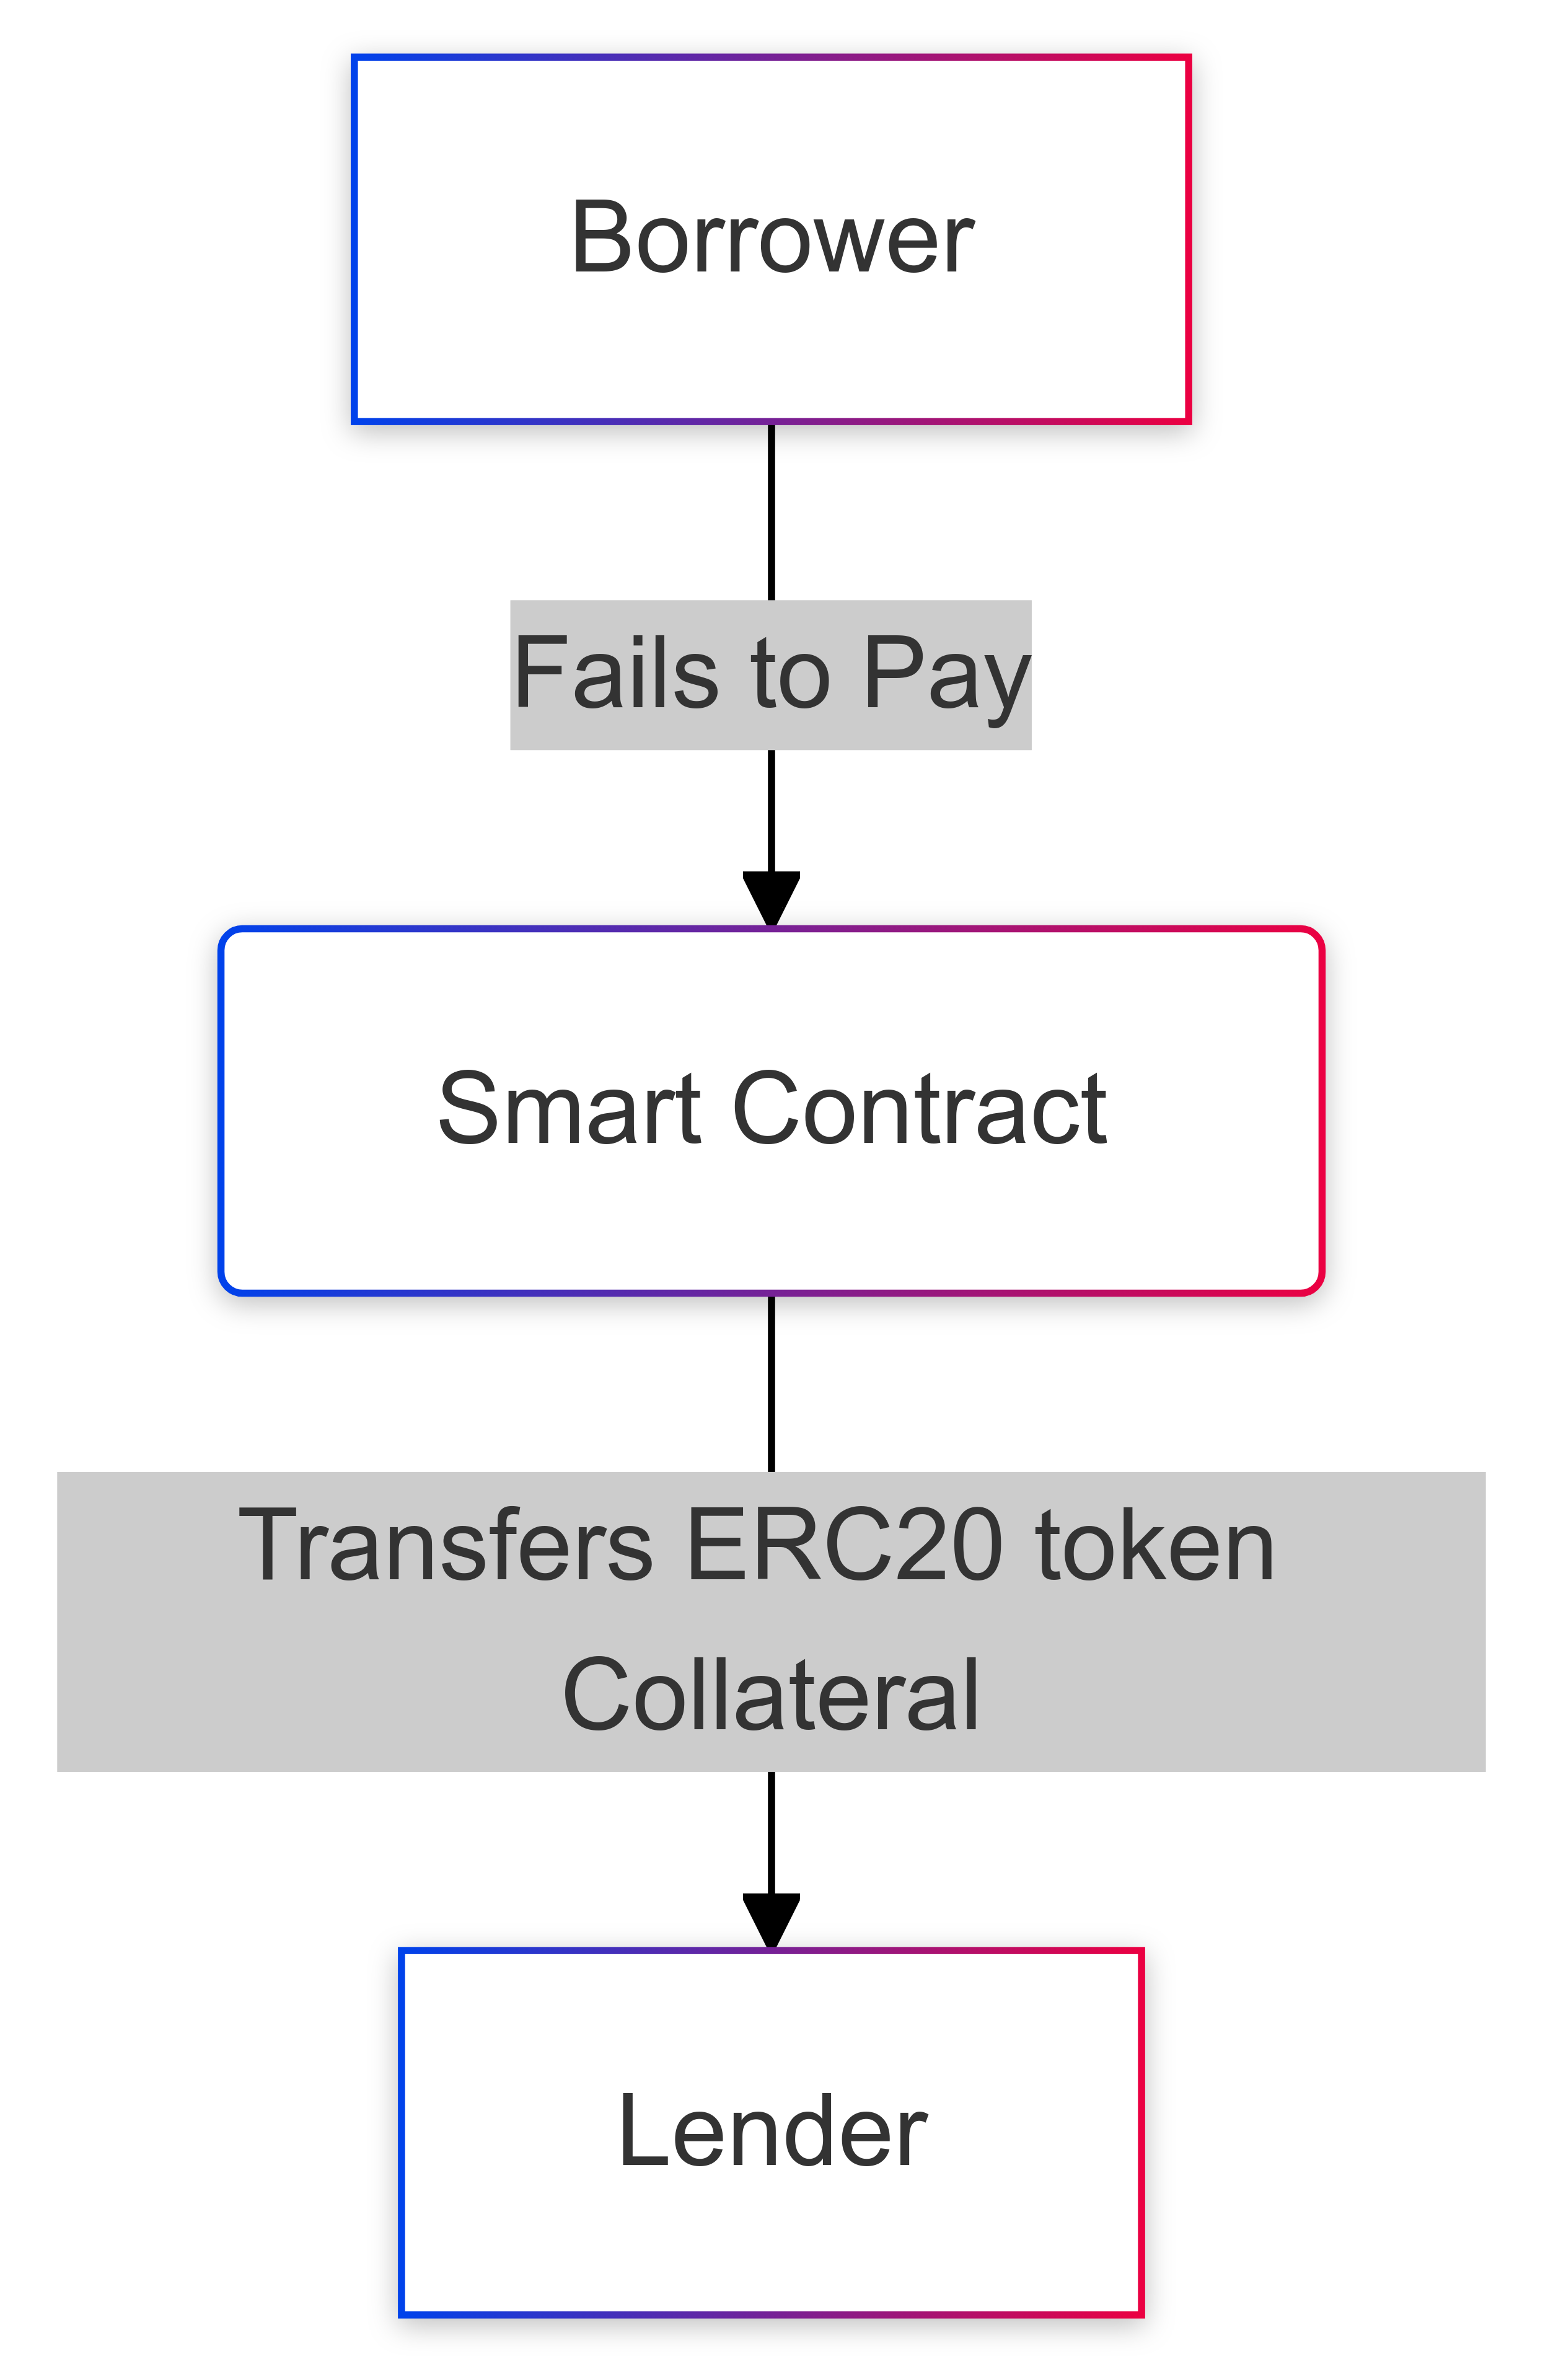
\includegraphics[width=\textwidth]{image/otcfailtopay}
        \caption{Borrower fails to repay the loan}
        \label{fig:fails}
    \end{minipage}
    \FloatBarrier
\end{figure}





Aave, from V1, breaks the P2P approach by creating lending pools where lenders deposit a cryptocurrency accepted by the protocol for the specific pool in exchange of a proxy token, receiving algorithmically calculated interest and borrowers borrow from the pool providing in exchange a collateral, chosen among the accepted ones from the protocol.
\begin{figure}[ht]
    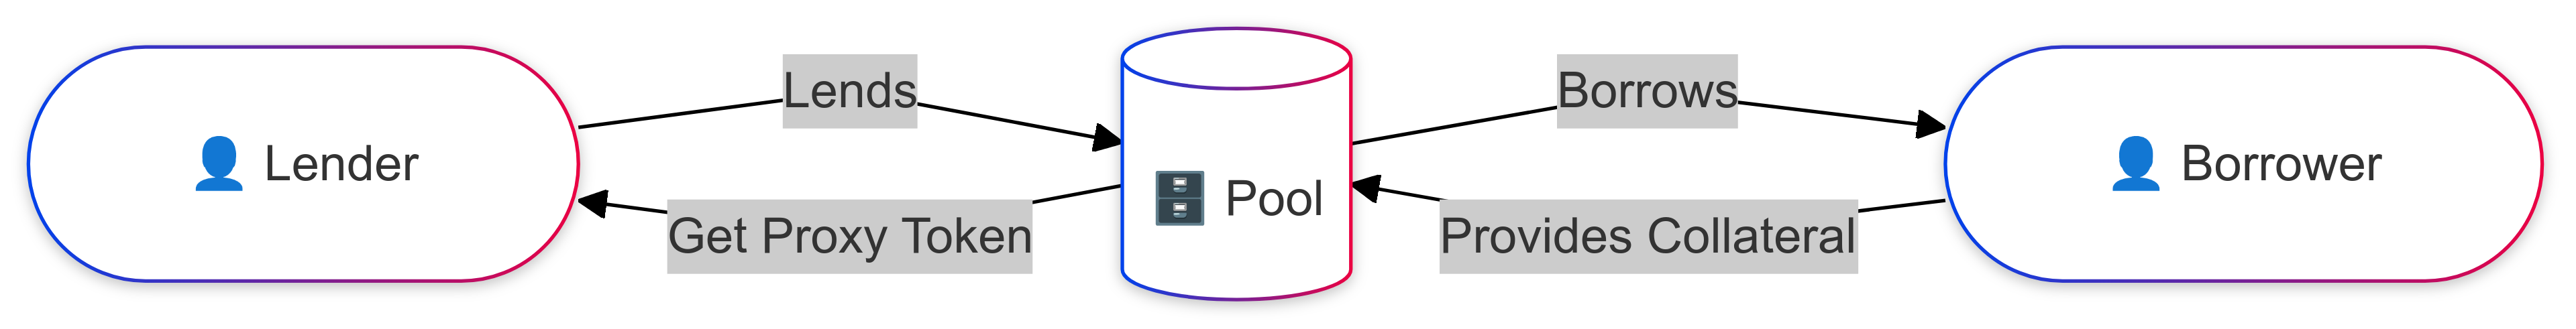
\includegraphics[width=0.7\textwidth]{image/lenderborrower.png}
    \caption{Aave standard lending borrowing}
\end{figure}
Borrowing can be at variable or fix rate and each borrowing position has an health factor ($H_f$) which potentially triggers, based on an algorithm, a liquidation for an under collateralised loan ($H_f$ below a calculated threshold). In traditional finance this can be similar to a margin call  with the addition of an upgradable protocol driving the calls based on mathematical functions proposed through a governance process.

\begin{table}[ht]
\centering
\caption{Comparison Between ethLend and Traditional Finance}
\begin{tabular}{ll}\toprule
\textbf{ethLend} & \textbf{Traditional Finance} \\ \midrule
Decentralized     & Centralized                \\
Peer-to-peer (P2P) & Over-the-counter (OTC)     \\
Fail to pay: Liquidation & Fail to pay: Collateral swap \\ \bottomrule
\end{tabular}\\
%%\text{\footnotesize{Comparison between Aave V1 and traditional finance}}
\label{tab:ethlend_vs_trad_fin}
\end{table}

Aave V2 enhance V1 as gives the possibility of upgrading the proxy tokens given to lenders, reduces gas inefficiencies and simplifies code and architecture.
V1 has the merit of flashloans introduction and V2 allows to use them for collateral trading, which means swapping collateral without closing and reopening a position, loan repayments, margin trading, debt swaps and margin deposits. In table  \ref{tab:ethlend_vs_trad_fin} and table
 \ref{tab:aave_v2_vs_trad_fin} traditional finance is compared to ethlend and Aave V2 showing how well known processes have been translated in DEFI. 

\begin{table}[ht]
\centering
\caption{Comparison Between Aave V2 and Traditional Finance}
\begin{tabular}{ll}\toprule
\textbf{Aave V2} & \textbf{Traditional Finance} \\ \midrule
Decentralized & Centralized \\
Lending pool & (Derivative) market \\
Decentralized assessment of collateral & Collateral rating \\
Health Factor ($H_f$) & Margin definition \\
Collateral adjustments to avoid liquidation & Collateral adjustments to avoid liquidation \\
$H_f$ close to 1: Alarm & Collateral $< $Margin: Margin call \\
Collateral increase or liquidation & Collateral increase or liquidation \\ \bottomrule
\end{tabular}\\
\text{\footnotesize{This table compares Aave V2 and traditional finance approaches in lending and collateral management.}}
\label{tab:aave_v2_vs_trad_fin}
\end{table}


\subsection{Aave Lending pool contract}

\begin{figure}[ht]
    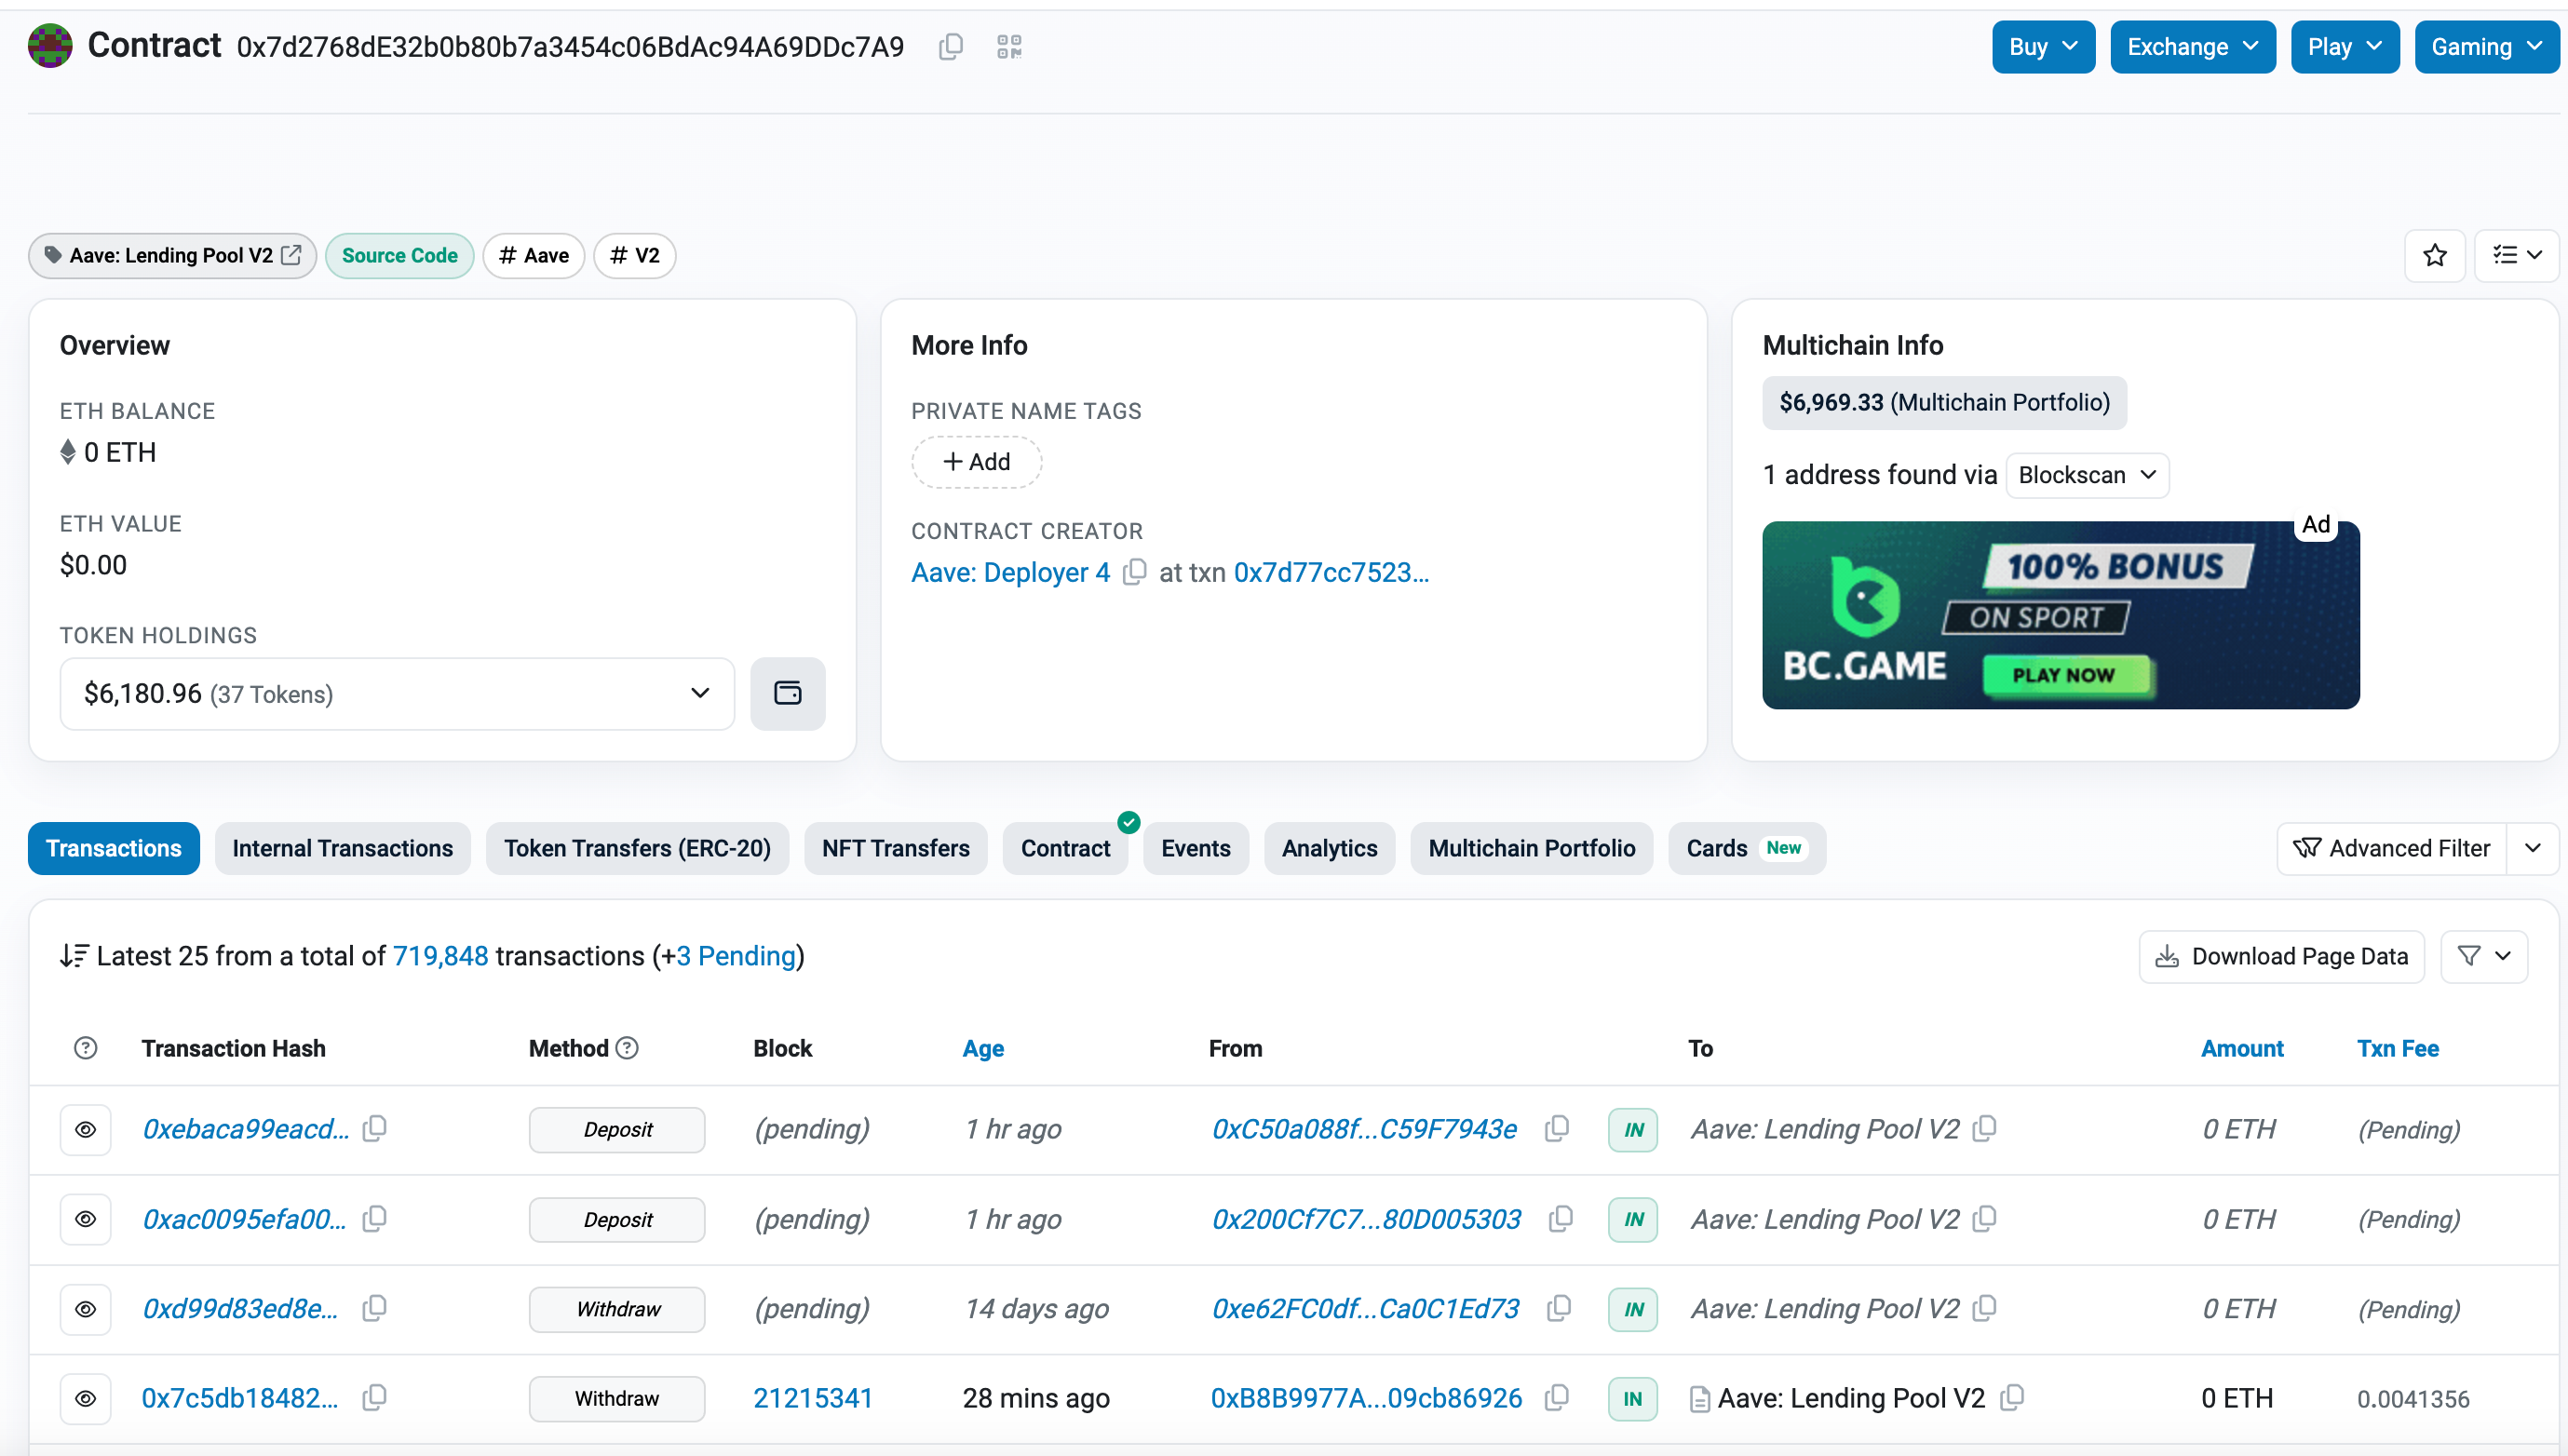
\includegraphics[width=1\textwidth]{image/etherscanLPool.png}
    \caption{Monitoring in etherscan Aave Lending Pool contract}
    \label{fig:etherscanLPool}
\end{figure}


A protocol based on ehtereum consists in a set of smart contracts. For the purpouse of Aave V2 flashloans a smart contract is handling the lending pool (including flashloan) calls. Such smart contract  is deployed on ethereum  as LendingPool  with contract address in ethereum main network: 0x7d2768dE32b0b80b7a3454c06BdAc94A69DDc7A9 which  includes calls which allow to deposit, redeem, borrow, repay, swap rate, liquidate, calling flash loans among others. This allows whoever has access to the ethereum blockchain to track the contract and the related transactions.

This paper  focus is on calls to LendingPool flashloan from ethereum inception to block number 20399999 correspondent to the date 27 July 2024.

\begin{table}[ht]
\centering
\caption{LendingPool Aave V2 Contract Methods}
\resizebox{\textwidth}{!}{%
\begin{tabular}{lll}\toprule
\textbf{Method Name} & \textbf{Synthetic Description} & \textbf{Keccak Selector} \\ \midrule
\texttt{deposit}     & Supply assets to the LendingPool to earn interest. & \texttt{0xe8eda9df} \\
\texttt{withdraw}    & Withdraw deposited assets from the pool.           & \texttt{0x6b91c3e7} \\
\texttt{borrow}      & Borrow assets from the pool against provided collateral. & \texttt{0x210dccae} \\
\texttt{repay}       & Repay a borrowed asset to restore collateral usage. & \texttt{0xb7ea3af4} \\
\texttt{swapBorrowRateMode} & Switch between stable and variable interest rates. & \texttt{0x95db9357} \\
\texttt{liquidationCall} & Liquidate undercollateralized positions in the pool. & \texttt{0x3bde6c10} \\
\texttt{flashLoan}   & Execute a flash loan with zero collateral requirements. & \texttt{0xee2e0890} \\ \bottomrule
\end{tabular}%
}
\caption*{\footnotesize This table summarizes key methods of the Aave V2 LendingPool contract, including their Keccak-encoded selectors.}
\label{tab:lendingpool_methods}
\end{table}

The table above includes keccak Selector info. This is the way the contract and method calls  are persisted on the blockchain.

\subsection {Flashloans}

When a loan is issued a lending protocol as well as in traditional finance is expecting a collateral or a cashflow as a guarantee. \uline{Flashloans are unique in the blockchain environment as they don't require neither a collateral nor a cash flow, provided that the loan is paid, interests included, within the same ethereum transaction. If the loan is not repaid the transaction is rolled back, at the cost for the borrower of the gas needed for processing the aborted transaction}. 
\begin{figure}[ht]
    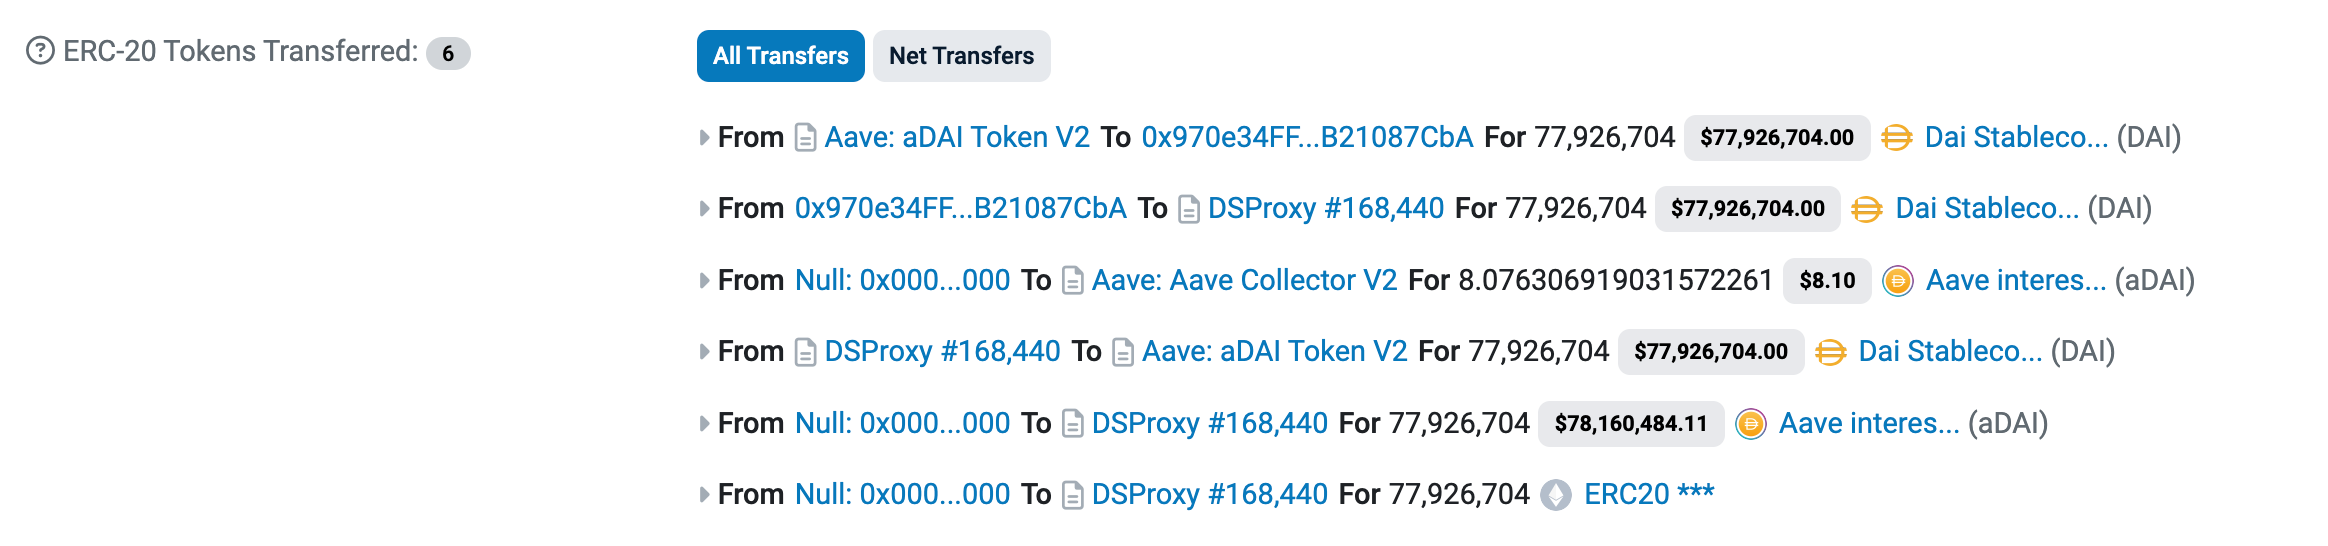
\includegraphics[width=1\textwidth]{image/flashloan.png}
    \caption{Example of a  flashloan}
    \label{fig:etherscanFLoan}
\end{figure}

The figure \ref{fig:etherscanFLoan} shows the transactions wrapped in a flashloan one. It is possible to recognize the opening of the loan (first transaction) and the repayment with interests (third and fourth transactions).






Flashloans are the main topic of this paper therefore is critical to clarify how they work. It is extremely common when reading documentation or articles to get confused by the statement that the repayment should happen within the same ethereum transaction: this can be misleading as with ethereum transaction, in this case is intended a transaction which can hold even hundreds of inner transactions as it is showed in Figure \ref{fig:etherscanFLoan}. This example shows a flashloan constituted of just six transactions as it has been chosen quite simple for the specific purpose.
It is common at this point to be confronted with the question how can many transactions be performed and, in some cases, rolled back.
To clarify this  it is crucial to recall the definition of transactions and block. Transactions are intended to be cryptographically signed instructions sent from one Ethereum account to another where the account can be a public address associated to private keys typically controlled by a person or a contract account associated to a smart contract and controlled by code, whereas a  block  is a component of the chain, containing among the others a set of transactions and the information to rebuild the chain itself. The nature of blockchain permits the creation of flashloans cause if a set of operations, in this case inner transaction within the flashloan one, is not ending with the full repayment, all the operations will be aborted by not being added to the block, therefore not ending in the blockchain. The flashloan is therefore computed in a precommit phase and the persistency in the blockchain is subordinated to the repayment plus interests.. The described behaviour leads to the creation which doesn't exists in traditional finance and is comparable to a rollback in a traditional relational database where the atomic operation is the full bunch of inner transaction wrapped by the flash loan one. 

\begin{table}[ht]
\centering
\caption{Comparison Between Flashloans and Databases}
\resizebox{\textwidth}{!}{%
\begin{tabular}{ll}\toprule
\textbf{Flashloans} & \textbf{Databases} \\ \midrule
Decentralized & Centralized \\
Open flashloan, inner transactions, repay flashloans & Begin transaction, internal transactions, end transaction \\
Add or not to the block & Commit or rollback \\
Block added to the chain & Persist operation in DB \\ \bottomrule
\end{tabular}%
}
\caption*{\footnotesize Flashloans have no counterpart in traditional finance. The best fit for a comparison is a transactional process in traditional databases.}
\label{tab:flashloans_vs_db}
\end{table}



Flashloans  are not enabling the user to get an infinite loan. The constraint are the liquidity of the pool, as a bigger amount than the pool size  itself cannot be accessed, and borrowing enabled for such pool.




\section{Self hosted Ethereum node}
\subsection {Introduction}
Ethereum is a distributed network of computers (known as nodes) running software that can verify blocks and transaction data. This is achieved by running on each computer of the network a client software which fullfills the ethereum specification. There are many implementation of such software and, provided that they fullfill all the protocol requirement, the nodes can interact independently from the  implementation they run. 
\begin{figure}[ht]
    \scalebox{1.4}{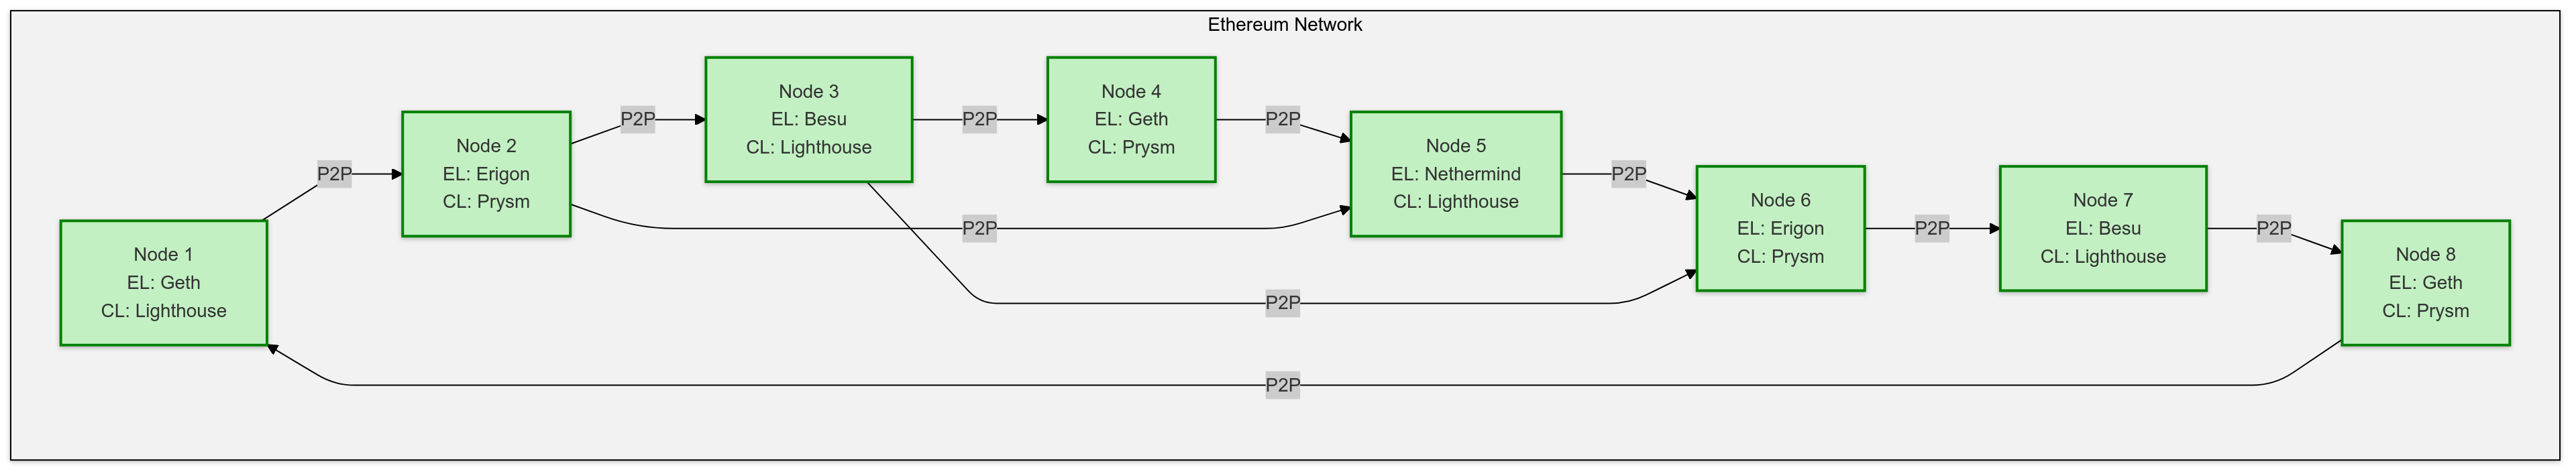
\includegraphics[width=0.7\textwidth]{image/simpleethnodes.png}}
    \caption{Symplified veiw of ethereum nodes}
    \label{fig:ethnodes}
\end{figure}

The figure \ref{fig:ethnodes} represents few nodes interacting. A node is any instance of Ethereum client software that is connected to other computers also running an Ethereum client software, forming a network. A client is an implementation of Ethereum that verifies data against the protocol rules and keeps the network secure. The figure \ref{fig:ethnodes} represents the current ethereum  state with a transition  from proof of work to proof of stake where a node has to run two clients, a consensus client and an execution client,  which come with different possible implementations. The execution client, also known as the Execution Engine, EL client or formerly the Eth1 client, listens to new transactions broadcasted in the network, executes them in EVM (Ethereum Virtual Machine), and holds the latest state and database of all current Ethereum data. The consensus client, also known as the Beacon Node, CL client or formerly the Eth2 client, implements the proof-of-stake consensus algorithm, which enables the network to achieve agreement based on validated data from the execution client. All these clients work together to keep track of the head of the Ethereum chain and allow users to interact with the Ethereum network. 

\subsection {Self hosted node vs provider}
This paper is written processing data from a self hosted node. That is not mandatory as it is possible to rely on services created ad hoc. Infura and Alchemy are popular third-party services that provide easy access to Ethereum nodes via APIs, allowing developers to interact with the Ethereum blockchain without running their own node. These services abstract the complexities of node management and provide scalable infrastructure for dApps, smart contract deployments, and blockchain analytics.
Using such services has the advantage of providing a standardised environment out of the box but comes with some disadvantages. On a bulk analysis API calls can get expensive, there is not a full control on the data accessed, the providers can block access and there are centralisation risks which are exacerbated by relying fully on third party providers.
Additionally externak providers implies  a lack of control on data while a node implementation gives both the control and tools for accessing such data: being this paper based on data analysis, the choice of a local node provider suitable to self hosting has been prioritised.
Running a node is not  trivial at the current stage of the ethereum network. An archive node can require more than 10 TB disk space with certain implementations, a good bandwidth, fast disks and a computer with 32 Gb Ram and multicore.
The next sections address the choice of node type and client implementation

% Table 1: Alchemy vs Infura
\begin{table}[ht]
\centering
\caption{Main characteristic Alchemy and Infura}
\resizebox{\textwidth}{!}{%
\begin{tabular}{ll}\toprule
\textbf{Alchemy} & \textbf{Infura} \\ \midrule
Advanced developer tools (e.g., debug API, enhanced APIs) & Basic Ethereum and IPFS API services \\
Performance optimizations (e.g., caching, load balancing) & Standard JSON-RPC API services \\
Customizable notifications and alerts & Basic webhook notifications \\
Higher-tier analytics for transaction debugging & Minimal analytics support \\
Enterprise-grade SLAs with premium support & Standard-tier SLAs \\ \bottomrule
\end{tabular}}
\label{tab:alchemy_vs_infura}
\end{table}

\begin{table}[ht]
\centering
\caption{Main characteristic Infura, Alchemy, and Self-Hosting a Node}
\resizebox{\textwidth}{!}{%
\begin{tabular}{p{0.3\textwidth} p{0.3\textwidth} p{0.3\textwidth}} \toprule
\textbf{Infura} & \textbf{Alchemy} & \textbf{Self-Hosting a Node} \\ \midrule
Cloud-hosted Ethereum and IPFS APIs & Enhanced APIs for analytics and debugging & Requires physical or virtual machine setup \\ \midrule
No need for hardware or sync maintenance & Managed infrastructure with performance optimizations & Full control over node and data \\ \midrule
Limited archive node access on basic plans & Advanced caching and query optimization & Can configure full or archive nodes as needed \\ \midrule
Third-party dependency & Dependency on Alchemy services & Full decentralization and sovereignty \\ \midrule
Quick and easy setup for development & Cloud-hosted, easy to scale & Longer setup time, requires technical expertise \\ \midrule
Usage limited by rate limits and quotas & Developer-focused tools (e.g., Notify API, transaction explorer) & Unlimited usage, depends on hardware capacity \\ \bottomrule
\end{tabular}}
\label{tab:infura_alchemy_self_hosting}
\end{table}


\subsection {Comparison of full nodes vs archive nodes in various ethereum implementations}

Ethereum nodes come in different types based on the amount of data they store and the roles they serve in the network. Running a self hosted node to perform data analysis requires to choose between a full node and an archive node.

A full node stores the complete current state of the Ethereum blockchain (i.e., account balances, contract storage, etc.) and recent historical data, but it prunes old state data to save space. Full nodes verify all transactions and blocks from the genesis block to the current state but don't keep every historical state like past balances or contract storage at every block.
An Archive Node stores everything that a full node does, but in addition, it keeps all historical states for every block in the blockchain. This means archive nodes can provide the exact state of the blockchain at any point in history, but they require significantly more disk space. Full nodes are sufficient for most operations, while archive nodes are only necessary to access to the entire historical state of the blockchain.


A full node stores enough information to partecipate to the ethereum network, also as validator, but data analysis would become cumbersome as the stored information is enough to rebuild and validate the current state but requires computation to do it: for this paper the archive node is therefore the best choice. 


\subsection {Motivation for choosing Erigon}


\begin{table}[H] % Use [H] to enforce placement
\centering
\caption{Resource Requirements for Ethereum Clients}
\resizebox{\textwidth}{!}{%
\begin{tabular}{lccccc}\toprule
\textbf{Client} & \textbf{Full Node Disk} & \textbf{Archive Node Disk} & \textbf{Full Node RAM} & \textbf{Archive Node RAM} & \textbf{CPU Requirements} \\ \midrule
Erigon & 400--500 GB & $\sim$3.5 TB & 2--8 GB & 8--16 GB & Optimized (low-medium) \\
Geth & 800--900 GB & $\sim$10 TB & 4--16 GB & 16 GB or more & High (sync heavy) \\
Besu & 800--900 GB & $\sim$10 TB & 8--16 GB & 16--32 GB & Medium \\
Nethermind & 700--900 GB & 6--8 TB & 4--8 GB & 16 GB or more & Optimized (medium) \\
Lighthouse, Prysm & 10--30 GB (Beacon) & N/A & 1--4 GB (Beacon) & N/A & Low \\ \bottomrule
\end{tabular}%
}
\captionsetup{font=footnotesize, justification=centering}
\caption*{\footnotesize This table lists the resource requirements for different Ethereum clients, including disk and RAM usage, and CPU demands for full and archive nodes.}
\label{tab:ethnodes}
\end{table}

There are many implementations of full archive nodes and the proper selection is related to  data analysis suitability: save disk space, fast access to data, a client which allow to present the data in an human readable format for easy interpretation. For this purpose  the most common implementations have been tested. The table  \ref{tab:ethnodes} summarises resource requirements for the most common node implementations. 
Geth is the most widely used Ethereum client, Erigon is designed to be more resource-efficient than traditional Geth, especially in terms of disk usage and sync time.
Besu is an Ethereum client written in Java, commonly used in enterprise environments.
Nethermind is a high-performance Ethereum client written in C\# with a focus on speed and configurability.
Besu and Geth may require more memory depending on the workload.

For the present purpose, a combination of Geth and Lighthouse was tested  (the latter only for consensus) as well as  Geth and Besu; the test of geth and besu aborted while the  second SSD disk installed as volume was half filled (max capacity 10 Tb and strong performance degradation).  Nevermind has not been tested as, being written in C\#, is strongly suboptimal to work on a linux instance: the data related to it are the result of a direct query with chatgpt (the documentation of these tool is tends not to be aligned with the development and therefore to underestimate the resources required: LINK TO DOC AND OFFICIAL STORAGE).
Considering the data presented in Table \ref{tab:ethnodes} Erigon looks the best fit, because it allows to run an archive node with a standard 4tb ssd disk. All ethereum node are very demanding in term of read write disk performance, therefore maximising the IO would be a plus, and two SSD in raid-0 are a good choice but not mandatory. 
\begin{figure}[ht]
    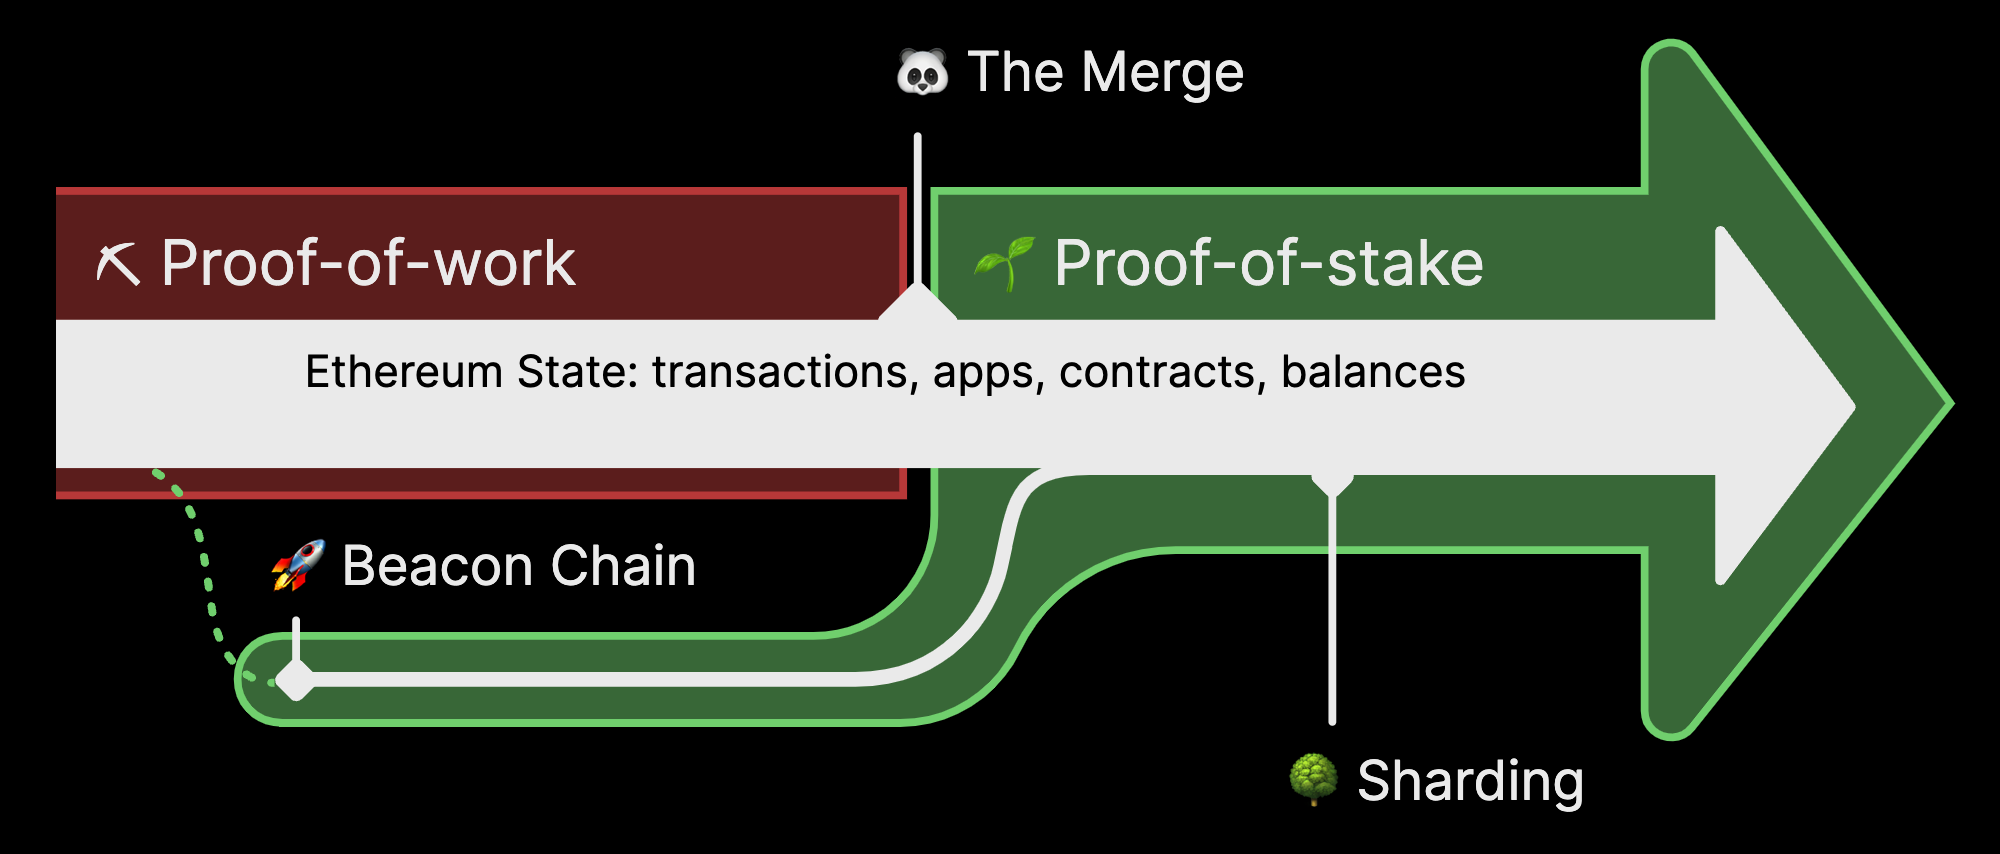
\includegraphics[width=0.7\textwidth]{image/powpos.png}
    \caption{Ethereum merge}
    \label{fig:powpos}
\end{figure}

Another advantage of Erigon is having an embedded consensus node implementation. Since the merge, which is represented in figure \ref{fig:powpos}, when ethereum became proof of stake, there is the need of an execution node and a consensus node. As showed in the picture for some time the consensus and execution layers run in parallel and they were consolidated in a unique chain with the merge; the consequence  for data analysis is that  the simplest is the consensus the best as the meaningful data are held in the execution layer. This is the case of caplin, the embedded consensus node in erigon, as it allows to achieve an archive node full synch without any configuration or installation of a compatible consensus node.
Before starting the work in the main chain  Erigon was tested on sepolia, a light test network, and verified that the data saved in a key value db, mdbx, were properly indexed and rendered by the embedded UI, otterscan. The last requirement for the analysis is being able to stop the synch at a certain block and run an rpc (remote procedure call) server which serves the data without synching continuously. Erigon satisfy also this. This allows to synch just once the main network till the desired block and then stop this operation, extremely resource demanding in term of bandwidth even when close to the ethereum chain tip.
An additional section addresses otterscan compared to other ethereum UI like etherscan and blockscout.
The table \ref{tab:adverigon} summarises erigon advantage for self hosted data analysis:


\begin{table}[ht]
\centering
\caption{Erigon Advantages for Data Analysis}
\begin{tabular}{cccc} \hline\hline
\textbf{Advantage} \\ \midrule
Embedded consensus \\
Low disk usage \\
Fast read \\
UI integrated \\
Geth tools available out of the box \\ \bottomrule
\end{tabular}\\
\text{\footnotesize{This table lists the key advantages of using Erigon for data analysis.}}
\label{tab:adverigon}
\end{table}

\section{Blockchain explorers}
\subsection{Blockchain explorer usage}
A blockchain explorer is a crucial tool for viewing, analyzing, and understanding data on a blockchain. It transforms complex, encoded information into human-readable form, making it easier to track transactions, verify addresses, explore smart contracts and can perform, in some case, some statistical analysis on behalf of the end user. Without a blockchain explorer, transaction data and smart contract interactions appear as hex-encoded information, which is not human-readable: below a set of pictures of a transaction in etherscan (the most used blockchain explorer), in otterscan (the explorer integrated in erigon) and raw data polling the node shows the difference between raw data and the same data rendered in an explorer  the importance of utilising properly an explorer or a combination of them.


FIGURES HERE AND COMMENTS


The pictures show the same transaction: calling a Uniswap contract to swap tokens.  An explorer decodes the data, showing details like token names, transfer amounts, and method names, so users can understand what actions are taking place.
the raw data instead look like a series of encoded hexadecimal strings. Decoding is done programmatically using a set of rules known as the Ethereum Application Binary Interface (ABI). The ABI defines how to encode and decode function names and parameters for Ethereum smart contracts, allowing a blockchain explorer or other tools to convert raw transaction data into human-readable formats. Several libraries make ABI decoding relatively straightforward, especially for developers building tools or explorers:  web3.js,  ethers.js, Web3.py.
For common contracts like Uniswap or ERC-20 tokens, the ABI files are usually public and can be added to the explorer's ABI database. These ABIs can be used to automatically identify functions and parameters, enabling accurate decoding.Blockchain explorers identify known smart contracts, such as Uniswap in the example above, by using their contract address and displaying relevant details, like contract name and functions. This allows users to recognise trusted contracts versus unknown ones, adding a layer of security when interacting with decentralized finance (DeFi) apps and other dApps.
Explorers like Etherscan and Otterscan can show verified source code and contract metadata (if available) to give insights into the contract’s purpose and functionality. In analysing a transaction sent to a Uniswap contract to perform a token swap the destination address (Uniswap’s contract) and the hex-encoded transaction data (e.g., `0x18cbafe5` followed by more data) couldn’t be interpreted easily. An explorer decodes this, revealing that `0x18cbafe5` maps to `swapExactTokensForTokens` and decodes other parameters, showing token addresses, amounts, and recipient addresses. 




In appendix xxx we show how to decode transactions in a purely programmatically way. This proofs the utility of explorers and shows what we nseed to do when explorer are not sufficient.
\subsection{Analyse tx in blockchain explorers}
Inhalt Inhalt Inhalt Inhalt Inhalt Inhalt Inhalt Inhalt Inhalt Inhalt Inhalt Inhalt Inhalt Inhalt Inhalt Inhalt Inhalt Inhalt Inhalt Inhalt Inhalt Inhalt Inhalt Inhalt Inhalt Inhalt Inhalt Inhalt Inhalt Inhalt Inhalt Inhalt Inhalt Inhalt Inhalt Inhalt Inhalt Inhalt Inhalt Inhalt Inhalt Inhalt Inhalt Inhalt Inhalt Inhalt Inhalt Inhalt Inhalt Inhalt Inhalt Inhalt Inhalt Inhalt Inhalt Inhalt Inhalt Inhalt Inhalt Inhalt Inhalt Inhalt Inhalt Inhalt Inhalt Inhalt Inhalt Inhalt Inhalt Inhalt Inhalt Inhalt Inhalt Inhalt Inhalt Inhalt Inhalt Inhalt Inhalt Inhalt Inhalt Inhalt Inhalt Inhalt Inhalt Inhalt Inhalt Inhalt Inhalt Inhalt Inhalt Inhalt Inhalt Inhalt Inhalt Inhalt Inhalt Inhalt Inhalt Inhalt Inhalt Inhalt Inhalt Inhalt Inhalt Inhalt Inhalt Inhalt Inhalt Inhalt Inhalt Inhalt Inhalt Inhalt Inhalt Inhalt Inhalt Inhalt Inhalt Inhalt Inhalt Inhalt Inhalt Inhalt Inhalt Inhalt Inhalt Inhalt Inhalt Inhalt Inhalt Inhalt Inhalt Inhalt Inhalt Inhalt Inhalt Inhalt Inhalt Inhalt Inhalt Inhalt Inhalt Inhalt Inhalt Inhalt Inhalt Inhalt Inhalt Inhalt Inhalt Inhalt Inhalt Inhalt Inhalt Inhalt Inhalt Inhalt Inhalt Inhalt Inhalt Inhalt Inhalt Inhalt Inhalt Inhalt Inhalt Inhalt Inhalt Inhalt Inhalt Inhalt Inhalt Inhalt Inhalt Inhalt Inhalt Inhalt Inhalt Inhalt Inhalt Inhalt Inhalt Inhalt Inhalt Inhalt Inhalt Inhalt Inhalt Inhalt Inhalt Inhalt Inhalt Inhalt Inhalt Inhalt Inhalt Inhalt Inhalt Inhalt Inhalt Inhalt Inhalt Inhalt Inhalt Inhalt Inhalt Inhalt Inhalt Inhalt Inhalt Inhalt Inhalt Inhalt Inhalt Inhalt Inhalt Inhalt Inhalt Inhalt  
\subsection{Explorer selection}
\subsection{Implikationen für Wissenschaft und Praxis}
Inhalt Inhalt Inhalt Inhalt Inhalt Inhalt Inhalt Inhalt Inhalt Inhalt Inhalt Inhalt Inhalt Inhalt Inhalt Inhalt Inhalt Inhalt Inhalt Inhalt Inhalt Inhalt Inhalt Inhalt Inhalt Inhalt Inhalt Inhalt Inhalt Inhalt Inhalt Inhalt Inhalt Inhalt Inhalt Inhalt Inhalt Inhalt Inhalt Inhalt Inhalt Inhalt Inhalt Inhalt Inhalt Inhalt Inhalt Inhalt Inhalt Inhalt Inhalt Inhalt Inhalt Inhalt Inhalt Inhalt Inhalt Inhalt Inhalt Inhalt Inhalt Inhalt Inhalt Inhalt Inhalt Inhalt Inhalt Inhalt Inhalt Inhalt Inhalt Inhalt Inhalt Inhalt Inhalt Inhalt Inhalt Inhalt Inhalt Inhalt Inhalt Inhalt Inhalt Inhalt Inhalt Inhalt Inhalt Inhalt Inhalt Inhalt Inhalt Inhalt Inhalt Inhalt Inhalt Inhalt Inhalt Inhalt Inhalt Inhalt Inhalt Inhalt Inhalt Inhalt Inhalt Inhalt Inhalt Inhalt Inhalt Inhalt Inhalt Inhalt Inhalt Inhalt Inhalt Inhalt Inhalt Inhalt Inhalt Inhalt Inhalt Inhalt Inhalt Inhalt Inhalt Inhalt Inhalt Inhalt Inhalt Inhalt Inhalt Inhalt Inhalt Inhalt Inhalt Inhalt Inhalt Inhalt Inhalt Inhalt Inhalt Inhalt Inhalt Inhalt Inhalt Inhalt Inhalt Inhalt Inhalt Inhalt Inhalt Inhalt Inhalt Inhalt Inhalt Inhalt Inhalt Inhalt Inhalt Inhalt Inhalt Inhalt Inhalt Inhalt Inhalt Inhalt Inhalt Inhalt Inhalt Inhalt Inhalt Inhalt Inhalt Inhalt Inhalt Inhalt Inhalt Inhalt Inhalt Inhalt Inhalt Inhalt Inhalt Inhalt Inhalt Inhalt Inhalt Inhalt Inhalt Inhalt Inhalt Inhalt Inhalt Inhalt Inhalt Inhalt Inhalt Inhalt Inhalt Inhalt Inhalt Inhalt Inhalt Inhalt Inhalt Inhalt Inhalt Inhalt Inhalt Inhalt Inhalt Inhalt Inhalt Inhalt Inhalt Inhalt Inhalt Inhalt Inhalt Inhalt Inhalt Inhalt Inhalt Inhalt Inhalt Inhalt Inhalt Inhalt Inhalt Inhalt Inhalt Inhalt Inhalt Inhalt Inhalt Inhalt Inhalt Inhalt Inhalt Inhalt Inhalt Inhalt Inhalt Inhalt Inhalt Inhalt Inhalt Inhalt Inhalt Inhalt Inhalt Inhalt Inhalt Inhalt Inhalt Inhalt Inhalt Inhalt Inhalt Inhalt Inhalt Inhalt Inhalt Inhalt Inhalt Inhalt Inhalt Inhalt Inhalt Inhalt Inhalt Inhalt Inhalt Inhalt Inhalt Inhalt Inhalt Inhalt Inhalt Inhalt Inhalt Inhalt Inhalt Inhalt Inhalt Inhalt Inhalt Inhalt Inhalt Inhalt Inhalt Inhalt Inhalt Inhalt Inhalt Inhalt Inhalt Inhalt Inhalt Inhalt Inhalt Inhalt Inhalt Inhalt Inhalt Inhalt Inhalt Inhalt Inhalt Inhalt Inhalt Inhalt Inhalt Inhalt Inhalt Inhalt Inhalt Inhalt Inhalt Inhalt 


\section{LAST CHAPTER ENDING WITH NEW PAGE}
\subsection{Blockchain explorer usage}
\subsection{Analyse tx in blockchain explorers}
Inhalt Inhalt Inhalt Inhalt Inhalt Inhalt Inhalt Inhalt Inhalt Inhalt Inhalt Inhalt Inhalt Inhalt Inhalt Inhalt Inhalt Inhalt Inhalt Inhalt Inhalt Inhalt Inhalt Inhalt Inhalt Inhalt Inhalt Inhalt Inhalt Inhalt Inhalt Inhalt Inhalt Inhalt Inhalt Inhalt Inhalt Inhalt Inhalt Inhalt Inhalt Inhalt Inhalt Inhalt Inhalt Inhalt Inhalt Inhalt Inhalt Inhalt Inhalt Inhalt Inhalt Inhalt Inhalt Inhalt Inhalt Inhalt Inhalt Inhalt Inhalt Inhalt Inhalt Inhalt Inhalt Inhalt Inhalt Inhalt Inhalt Inhalt Inhalt Inhalt Inhalt Inhalt Inhalt Inhalt Inhalt Inhalt Inhalt Inhalt Inhalt Inhalt Inhalt Inhalt Inhalt Inhalt Inhalt Inhalt Inhalt Inhalt Inhalt Inhalt Inhalt Inhalt Inhalt Inhalt Inhalt Inhalt Inhalt Inhalt Inhalt Inhalt Inhalt Inhalt Inhalt Inhalt Inhalt Inhalt Inhalt Inhalt Inhalt Inhalt Inhalt Inhalt Inhalt Inhalt Inhalt Inhalt Inhalt Inhalt Inhalt Inhalt Inhalt Inhalt Inhalt Inhalt Inhalt Inhalt Inhalt Inhalt Inhalt Inhalt Inhalt Inhalt Inhalt Inhalt Inhalt Inhalt Inhalt Inhalt Inhalt Inhalt Inhalt Inhalt Inhalt Inhalt Inhalt Inhalt Inhalt Inhalt Inhalt Inhalt Inhalt Inhalt Inhalt Inhalt Inhalt Inhalt Inhalt Inhalt Inhalt Inhalt Inhalt Inhalt Inhalt Inhalt Inhalt Inhalt Inhalt Inhalt Inhalt Inhalt Inhalt Inhalt Inhalt Inhalt Inhalt Inhalt Inhalt Inhalt Inhalt Inhalt Inhalt Inhalt Inhalt Inhalt Inhalt Inhalt Inhalt Inhalt Inhalt Inhalt Inhalt Inhalt Inhalt Inhalt Inhalt Inhalt Inhalt Inhalt Inhalt Inhalt Inhalt Inhalt Inhalt Inhalt Inhalt Inhalt Inhalt Inhalt Inhalt Inhalt Inhalt Inhalt Inhalt Inhalt Inhalt Inhalt Inhalt Inhalt  
\subsection{Explorer selection}
\subsection{Implikationen für Wissenschaft und Praxis}
Inhalt Inhalt Inhalt Inhalt Inhalt Inhalt Inhalt Inhalt Inhalt Inhalt Inhalt Inhalt Inhalt Inhalt Inhalt Inhalt Inhalt Inhalt Inhalt Inhalt Inhalt Inhalt Inhalt Inhalt Inhalt Inhalt Inhalt Inhalt Inhalt Inhalt Inhalt Inhalt Inhalt Inhalt Inhalt Inhalt Inhalt Inhalt Inhalt Inhalt Inhalt Inhalt Inhalt Inhalt Inhalt Inhalt Inhalt Inhalt Inhalt Inhalt Inhalt Inhalt Inhalt Inhalt Inhalt Inhalt Inhalt Inhalt Inhalt Inhalt Inhalt Inhalt Inhalt Inhalt Inhalt Inhalt Inhalt Inhalt Inhalt Inhalt Inhalt Inhalt Inhalt Inhalt Inhalt Inhalt Inhalt Inhalt Inhalt Inhalt Inhalt Inhalt Inhalt Inhalt Inhalt Inhalt Inhalt Inhalt Inhalt Inhalt Inhalt Inhalt Inhalt Inhalt Inhalt Inhalt Inhalt Inhalt Inhalt Inhalt Inhalt Inhalt Inhalt Inhalt Inhalt Inhalt Inhalt Inhalt Inhalt Inhalt Inhalt Inhalt Inhalt Inhalt Inhalt Inhalt Inhalt Inhalt Inhalt Inhalt Inhalt Inhalt Inhalt Inhalt Inhalt Inhalt Inhalt Inhalt Inhalt Inhalt Inhalt Inhalt Inhalt Inhalt Inhalt Inhalt Inhalt Inhalt Inhalt Inhalt Inhalt Inhalt Inhalt Inhalt Inhalt Inhalt Inhalt Inhalt Inhalt Inhalt Inhalt Inhalt Inhalt Inhalt Inhalt Inhalt Inhalt Inhalt Inhalt Inhalt Inhalt Inhalt Inhalt Inhalt Inhalt Inhalt Inhalt Inhalt Inhalt Inhalt Inhalt Inhalt Inhalt Inhalt Inhalt Inhalt Inhalt Inhalt Inhalt Inhalt Inhalt Inhalt Inhalt Inhalt Inhalt Inhalt Inhalt Inhalt Inhalt Inhalt Inhalt Inhalt Inhalt Inhalt Inhalt Inhalt Inhalt Inhalt Inhalt Inhalt Inhalt Inhalt Inhalt Inhalt Inhalt Inhalt Inhalt Inhalt Inhalt Inhalt Inhalt Inhalt Inhalt Inhalt Inhalt Inhalt Inhalt Inhalt Inhalt Inhalt Inhalt Inhalt Inhalt Inhalt Inhalt Inhalt Inhalt Inhalt Inhalt Inhalt Inhalt Inhalt Inhalt Inhalt Inhalt Inhalt Inhalt Inhalt Inhalt Inhalt Inhalt Inhalt Inhalt Inhalt Inhalt Inhalt Inhalt Inhalt Inhalt Inhalt Inhalt Inhalt Inhalt Inhalt Inhalt Inhalt Inhalt Inhalt Inhalt Inhalt Inhalt Inhalt Inhalt Inhalt Inhalt Inhalt Inhalt Inhalt Inhalt Inhalt Inhalt Inhalt Inhalt Inhalt Inhalt Inhalt Inhalt Inhalt Inhalt Inhalt Inhalt Inhalt Inhalt Inhalt Inhalt Inhalt Inhalt Inhalt Inhalt Inhalt Inhalt Inhalt Inhalt Inhalt Inhalt Inhalt Inhalt Inhalt Inhalt Inhalt Inhalt Inhalt Inhalt Inhalt Inhalt Inhalt Inhalt Inhalt Inhalt Inhalt Inhalt Inhalt Inhalt Inhalt Inhalt Inhalt Inhalt Inhalt Inhalt Inhalt 


\newpage
\section{Literaturverzeichnis}
Gantenbein, Pascal, und Marco Gehrig, 2007, Moderne Unternehmensbewertung, \textit{Der
Schweizer Treuhänder}, S. 602 – 612.


\newpage
\section{Anhang}
\subsection*{Eidesstattliche Erklärung}
Hiermit erkläre ich, dass ich die vorliegende Arbeit selbständig und ohne Benutzung anderer als der angegebenen Hilfsmittel angefertigt habe. Mir ist bekannt, dass ich die volle Verantwortung für die Wissenschaftlichkeit des vorgelegten Textes selbst übernehme, auch wenn KI-Hilfsmittel eingesetzt und deklariert wurden. Alle Stellen, die wörtlich oder sinngemäss aus veröffentlichten oder nicht veröffentlichten Schriften entnommen wurden, sind als solche kenntlich gemacht. Die Arbeit ist in gleicher oder ähnlicher Form oder auszugsweise im Rahmen einer anderen Prüfung noch nicht vorgelegt worden.\\\\\
\noindent Ort, den XX.XX.20YY
\begin{flushright}
$\overline{~~~~~~~~~\mbox{(Unterschrift der Verfasserin)}~~~~~~~~~}$
\end{flushright}

\end{document}  



